\subsection{Mitocondria Striatum}
For the Mitocondria Striatum set, CNN are employed to solve a segmentation problem. Every pixel is classified as being part of the mitocondria or not. A patch of 51x51 surrounding the pixel is extracted from the image and fed as input to a CNN which acts as a binary classifier. For determining the parameters of the CNN we used a set of
100.000 samples for training and 20.000 for validation (containing half positive and half negative samples). After determining the best setup, the network was trained on a larger set of 1 milion samples for training and 200.000 for validation.

The final test data represented a 3D image volume consisting of 318 slices of size 400x661. Thus, one frame contains 264.400 datasamples that are fed as test input for the CNN, while all frames contain 97 million datasamples.

The best setup obtained using the small training and validation set was the one presented in Fig\ref{fig:CNN3} NonSep. This gave us a VOC error on the first frame of 77.2. We then trained this net on the big set and obtained an error of 74. We notice that this is not comparable with state of the art methods which achieve results higher than 79 VOC or that use 3D information. The goal of this
is to see if we can obtain a speedup by using separable filters.
\begin{table}
\centering
\begin{tabular}{@{}rlll@{}}\toprule
Layer & Type & Maps and neurons& Kernel size \\ \midrule
0 & input & 1 map of 51x51 &\\
1& convolutional & 10 maps of 46x46 & 6x6\\
2 & max pooling & 10 maps of 23x23 &  \\
3 & convolutional & 20 maps of 18x18& 6x6 \\
4 & max pooling & 20 maps of 9x9& \\ 
3 & convolutional & 50 maps of 4x4& 6x6 \\
4 & max pooling & 50 maps of 2x2& \\ 
5 & fully conntected& 100 & \\
6 & fully conntected & 2 neurons & \\ \bottomrule
\end{tabular}
\caption{CNN for Mitocondria set}
\label{fig:CNN3}
\end{table}
Example of the weights learned in the first convolutional layer are shown in Fig[ref] and of output on one frame produced by the CNN. 
\begin{table}
\centering
\begin{tabular}{@{}rllll@{}}\toprule
 &&Conv L1& Conv L2 & Conv L3\\ \midrule
NonSep &Kernel Size & 10 maps 6x6& 20 maps 6x6 & 50 maps 6x6\\
&Speedup rank& $\leq$16.36 & $\leq$22.5 & $\leq$29.03\\
&Theoretical rank & 16.4 & $\leq$36 & 36 \\ 
&time & 8.1 & 26.8 & 18.4 \\ \midrule
Separable& rank & - & 20 & 36 \\ 
& time& - & 20.1 & 17.6\\ \midrule
\end{tabular}
\caption{CNN for Mitocondria set}
\label{fig:CNN3}
\end{table}
\begin{figure}[h!]
  \centering
  \begin{subfigure}[b]{0.40\textwidth}
   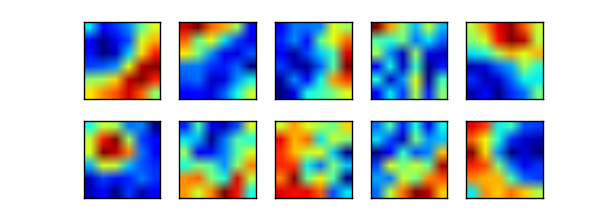
\includegraphics[width=\textwidth]{images/filters.png}
    \caption{Weights learned in the 1st layer}
  \end{subfigure}
  \begin{subfigure}[b]{0.40\textwidth}
    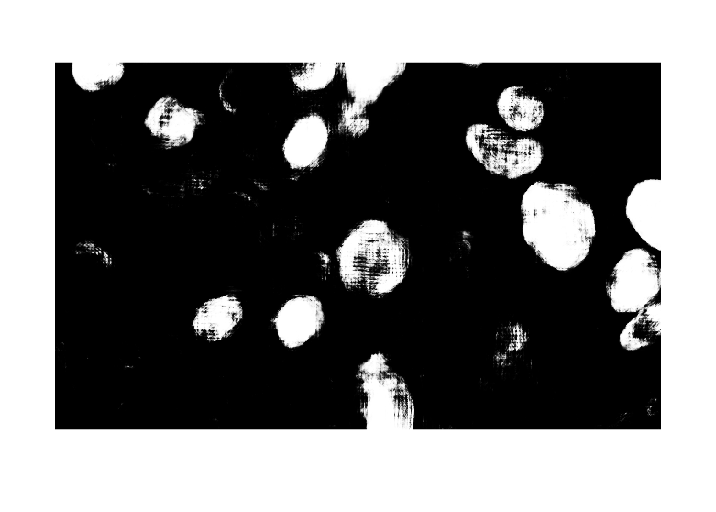
\includegraphics[width=\textwidth]{images/frame1.png}
    \caption{CNN output frame, not thresholded}
  \end{subfigure}
    \begin{subfigure}[b]{0.40\textwidth}
   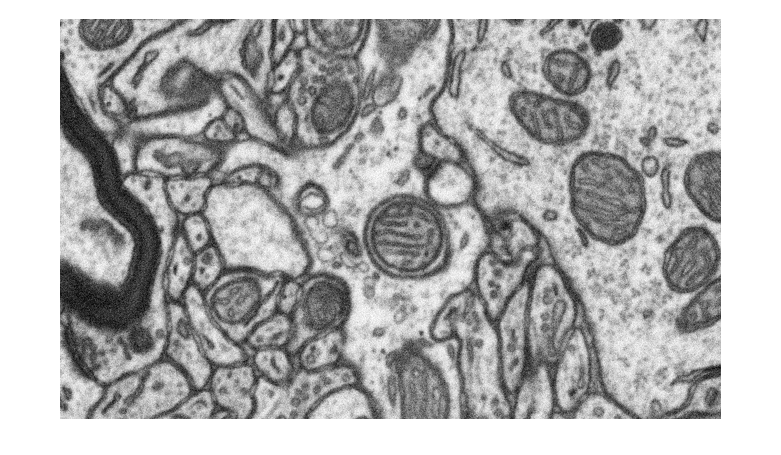
\includegraphics[width=\textwidth]{images/GT_truth.png}
    \caption{CNN input frame}
  \end{subfigure}
  \begin{subfigure}[b]{0.40\textwidth}
    
\includegraphics[width=\textwidth]{images/GTframe1.png}
    \caption{Groundtruth frame}
  \end{subfigure}
  \caption{Input and output example of CNN for mitocondria dataset. Fig a) shows that the filters are mostly edge and circle detectors which constitute basic building blocks for the interior of the mitocondria.
  Comparing b), c) and d) we notice the 'noisy' nature of the CNN output for pixel classification. Preprocessing the final output b) using a median filter would likely improve the results.}
  \label{fig:mitocondria}
\end{figure}
We keep conv L1 fixed and approximate conv L2 and L3 with rank 20 and 36 respectively. For the 3rd layer no significant change in performance is observed, while for layer 2 we notice a small speedup from roughly 26 to 20 ms. Since the fit of the two layers was very good (99.9) there was no drop in classification performance.

Fig \ref{fig:mitocondria} shows an example of the CNN input and output and the type of filters that it learns. 
